\section{Минимальные требования для класса <<Граф>>}
\subsection{Условие задания}
Для решения всех задач курса необходимо создать класс (или иерархию
классов "--- на усмотрение разработчика), содержащий:
\begin{enumerate}
  \item Структуру для хранения списка смежности графа (не работать с графом
  через матрицы смежности, если в некоторых алгоритмах удобнее использовать
  список ребер "--- реализовать метод, создающий список ребер на
  основе списка смежности).
  \item Конструкторы (не менее 3"~х):
  \begin{itemize}
    \item добавляющие вершину;
    \item добавляющие ребро (дугу);
    \item удаляющие вершину;
    \item удаляющие ребро (дугу);
    \item выводящие список смежности в файл (в том числе в пригодном для
    чтения конструктором формате).
  \end{itemize}
  \item Методы:
  \begin{itemize}
    \item конструктор по умолчанию, создающий пустой граф;
    \item конструктор, заполняющий данные графа из файла;
    \item конструктор"=копию (аккуратно, не все сразу делают именно копию);
    \item специфические конструкторы для удобства тестирования.
  \end{itemize}
  \item Должны поддерживаться как ориентированные, так и неориентированные
  графы.
  \item Добавьте минималистичный консольный интерфейс пользователя, позволяющий
  добавлять и удалять вершины и ребра (дуги) и просматривать
  текущий список смежности графа.
\end{enumerate}

\subsection{Примеры исходного кода}
Следующий код описывает класс \mitext{Graph}, соответствующий требованиям
условия:
\begin{minted}{typescript}
export class Graph {
  private adj: Map<string, Map<string, number>> = new Map()
  private weighted: boolean = false
  private oriented: boolean = false

  constructor(weighted: boolean, oriented: boolean)
  constructor(textRepr: string)
  constructor(other: Graph)
  constructor(arg1: boolean | string | Graph, arg2?: boolean) {
    if (typeof arg1 === 'boolean' && typeof arg2 === 'boolean') {
      this.weighted = arg1
      this.oriented = arg2
      this.adj = new Map()
    } else if (typeof arg1 === 'string' && arg2 == null) {
      this.loadFromFile(arg1)
      if (!this.oriented) {
        for (const [v, neighbors] of this.adj) {
          for (const [u, w] of neighbors) {
            this.adj.get(u)!.set(v, w)
          }
        }
      }
    } else if (arg1 instanceof Graph && arg2 == null) {
      this.weighted = arg1.weighted
      this.oriented = arg1.oriented
      this.adj = new Map(arg1.adj)
    } else {
      throw new Error('Invalid arguments')
    }
  }
  // другие методы ...
}
\end{minted}

Методы для добавления вершины и ребра (дуги):
\begin{minted}{typescript}
addNode(label: string) {
  if (this.adj.has(label)) {
    throw new NodeAlreadyExists(label)
  }
  this.adj.set(label, new Map())
}

connect(a: string, b: string, weight?: number) {
  if (!this.adj.has(a)) {
    throw new NodeNotExists(a)
  }
  if (!this.adj.has(b)) {
    throw new NodeNotExists(b)
  }
  if (this.adj.get(a)!.has(b)) {
    throw new ConnectionAlreadyExists(a, b)
  }

  if (this.weighted) {
    this.adj.get(a)!.set(b, weight!)
    if (!this.oriented) {
      this.adj.get(b)!.set(a, weight!)
    }
  } else {
    if (weight) {
      throw new WeightsInNonWeightedGraph()
    }
    this.adj.get(a)!.set(b, 0)
    if (!this.oriented) {
      this.adj.get(b)!.set(a, 0)
    }
  }
}
\end{minted}

Удаление вершины и дуги (ребра):
\begin{minted}{typescript}
removeNode(label: string) {
  if (!this.adj.has(label)) {
    throw new NodeNotExists(label)
  }

  this.adj.delete(label)
  for (let value of this.adj.values()) {
    value.delete(label)
  }
}

disconnect(a: string, b: string) {
  if (!this.adj.has(a)) {
    throw new NodeNotExists(a)
  }
  if (!this.adj.has(b)) {
    throw new NodeNotExists(b)
  }
  if (!this.adj.get(a)!.has(b)) {
    throw new ConnectionNotExists(a, b)
  }

  this.adj.get(a)!.delete(b)
  if (!this.oriented) {
    this.adj.get(b)!.delete(a)
  }
}
\end{minted}

\begin{figure}[H]
  \centering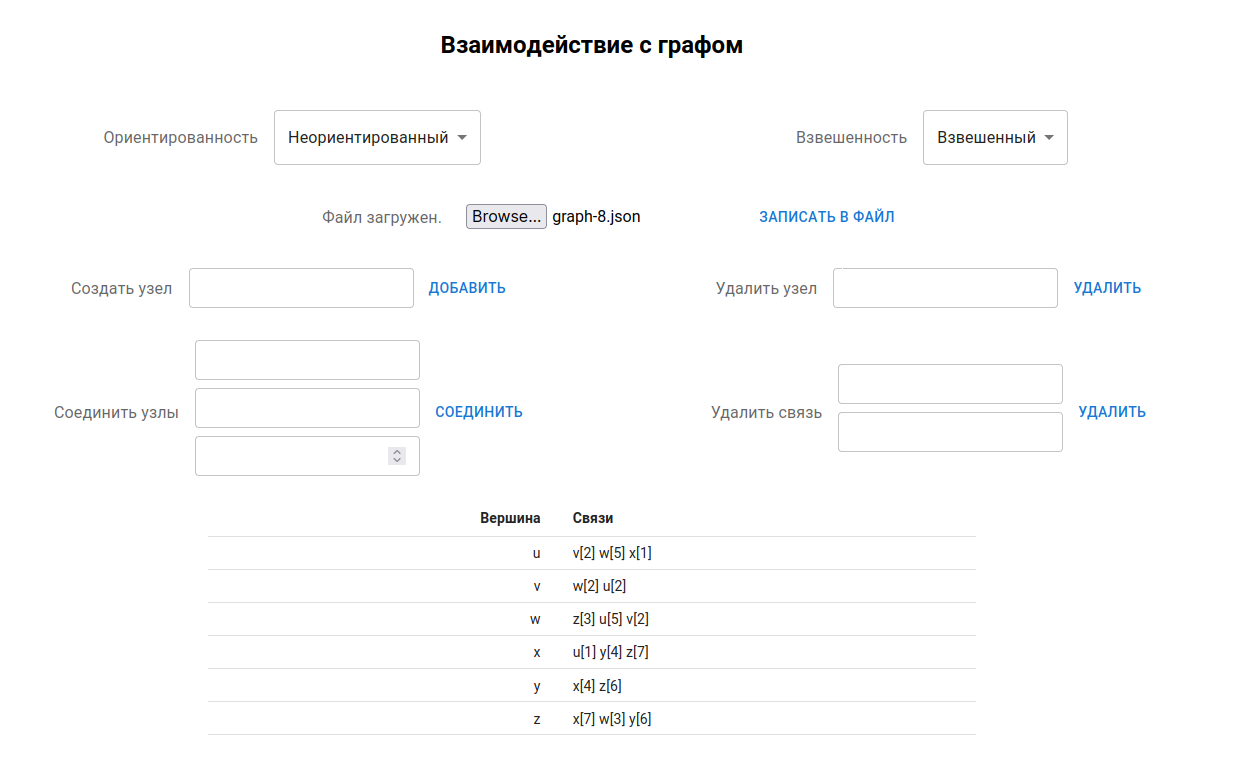
\includegraphics[width=1.0\textwidth]{figs/task-1/int-1.png}
  \caption{Общий вид интерфейса}
  \label{fig:int-overview}
\end{figure}

Вместо консольного был реализован веб"=интерфейс (см.\,рис.\,\ref{fig:int-overview})
на React.js. Основной компонент интерфейса (\mitext{App}) представлен в приложении
\ref{app:app-component}.

\begin{figure}[H]
  \begin{minipage}{0.5\textwidth}
    \centering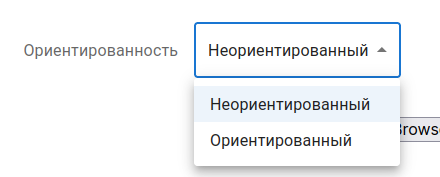
\includegraphics[width=0.7\linewidth]{figs/task-1/int-2.png}
  \end{minipage}
  \begin{minipage}{0.5\textwidth}
    \centering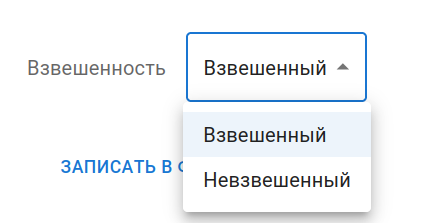
\includegraphics[width=0.7\linewidth]{figs/task-1/int-3.png}
  \end{minipage}
  \caption{Виды графов}
  \label{fig:int-basic-params}
\end{figure}

\begin{figure}
  \centering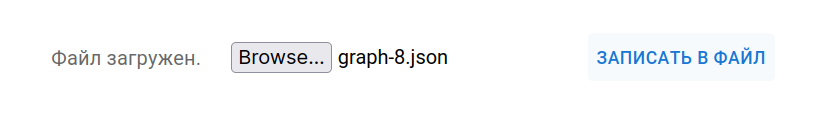
\includegraphics[width=0.8\textwidth]{figs/task-1/int-6.png}
  \caption{Загрузка и выгрузка в файл}
  \label{fig:int-file-io}
\end{figure}

Графы можно загружать из файлов и сохранять в файлы. В последнем случае
на компьютер скачается файл с описанием графа в формате JSON.

Интерфейс позволяет пользователю работать с различными видами графов:
ориентированным/неориентированным, взвешенным/невзвешенным\\
(см.\,рис.\,\ref{fig:int-basic-params}).

Текущее состояние графа отображается в виде списка смежности внизу
интерфейса.

Доступные операции:
\begin{itemize}
  \item добавление вершин;
  \item удаление вершин;
  \item создание связей;
  \item удаление связей.
\end{itemize}

\begin{figure}
  \begin{minipage}{0.5\textwidth}
    \centering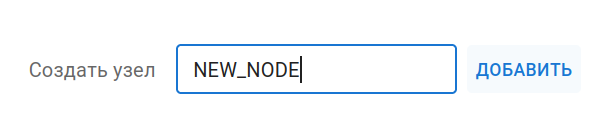
\includegraphics[width=0.8\linewidth]{figs/task-1/int-4.png}
  \end{minipage}
  \begin{minipage}{0.5\textwidth}
    \centering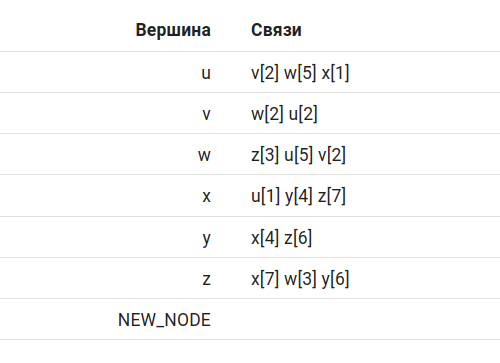
\includegraphics[width=0.7\linewidth]{figs/task-1/int-5.png}
  \end{minipage}
  \caption{Добавление вершины в граф}
  \label{fig:int-node-add}
\end{figure}

Пример добавления вершины и результат действия представлен на
рис.\,\ref{fig:int-node-add}.

\begin{figure}
  \begin{minipage}{0.5\textwidth}
    \centering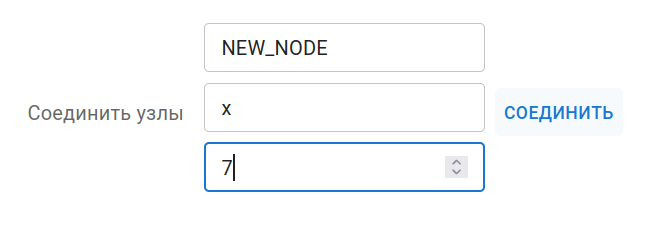
\includegraphics[width=0.8\linewidth]{figs/task-1/int-12.png}
  \end{minipage}
  \begin{minipage}{0.5\textwidth}
    \centering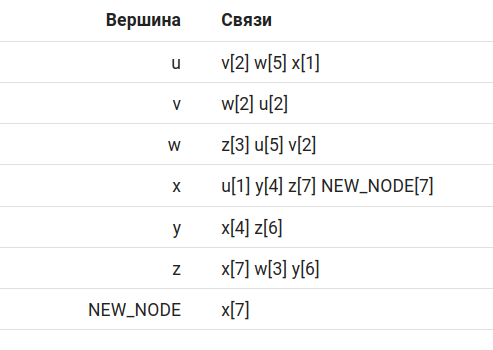
\includegraphics[width=0.8\linewidth]{figs/task-1/int-8.png}
  \end{minipage}
  \caption{Создание связи между вершинами}
  \label{fig:int-connect-nodes}
\end{figure}

Пример создания связи между вершинами и результат представлены
на рис.\,\ref{fig:int-connect-nodes}.

\begin{figure}
  \begin{minipage}{0.5\textwidth}
    \centering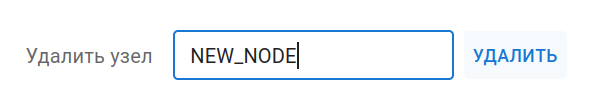
\includegraphics[width=0.8\linewidth]{figs/task-1/int-9.png}
  \end{minipage}
  \begin{minipage}{0.5\textwidth}
    \centering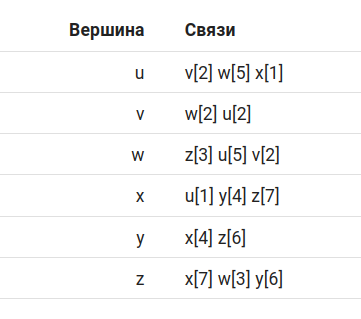
\includegraphics[width=0.8\linewidth]{figs/task-1/int-10.png}
  \end{minipage}
  \caption{Удаление вершины}
  \label{fig:int-node-del}
\end{figure}

Пример удаления вершины и результат представлены
на рис.\,\ref{fig:int-node-del}.

\begin{figure}
  \begin{minipage}{0.5\textwidth}
    \centering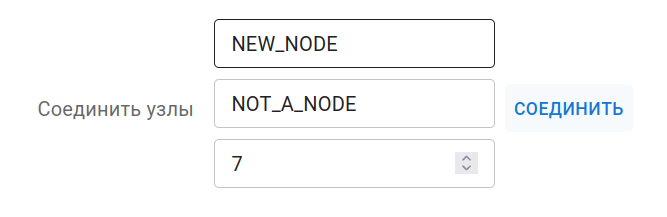
\includegraphics[width=0.7\linewidth]{figs/task-1/int-7.png}
  \end{minipage}
  \begin{minipage}{0.5\textwidth}
    \centering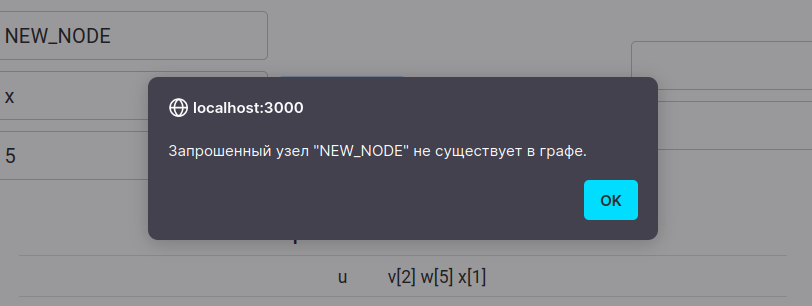
\includegraphics[width=0.8\linewidth]{figs/task-1/int-11.png}
  \end{minipage}
  \caption{Вывод сообщения об ошибке}
  \label{fig:int-alert}
\end{figure}

Если в какой"~то операции пользователь пытается выполнить недопустимое действие
(создать вершину с пустой меткой, сослаться на несуществующую вершину),
ему выводится сообщение об ошибке (см.\,рис.\,\ref{fig:int-alert}).

\subsection{Примеры входных и выходных данных}
Взвешенный ориентированный граф:
\begin{minted}{js}
{
  "weighted": true,
  "oriented": true,
  "adj": {
    "a": {
      "b": 2,
      "c": 3
    },
    "b": {
      "d": 5
    },
    "c": {
      "e": 4,
      "f": 2
    },
    "d": {
      "g": 6
    },
    "e": {
      "h": 3
    },
    "f": {
      "h": 7
    },
    "g": {
      "h": 8
    },
    "h": {}
  }
}
\end{minted}

Взвешенный неориентированный граф:
\begin{minted}{js}
{
  "weighted": true,
  "oriented": false,
  "adj": {
    "a": {
      "b": 2,
      "c": 3,
      "d": 5
    },
    "b": {
      "c": 4,
      "e": 6
    },
    "c": {
      "d": 1,
      "f": 3
    },
    "d": {
      "g": 2
    },
    "e": {
      "f": 4,
      "h": 5
    },
    "f": {
      "h": 2,
      "g": 3
    },
    "g": {
      "h": 1
    },
    "h": {}
  }
}
\end{minted}

Выходные файлы имеют такой же формат и полностью совместимы с входными.
